\documentclass[../main.tex]{subfiles}
\begin{document}

\section{Stand der Technik}

\subsection{Additive Fertigung}

Additive Fertigung, unabhängig von dem Werkstoff, ist ein Bereich im dem viel
geforscht und innoviert wird. In fast jedem Industriebereich wird versucht ein
bestehendes Design oder Modell zu optimieren und verbessern.
Sei es hinsichtlich Qualität oder Kosteneffizienz. Additive Fertigung bietet bei 
dieser Optimierung viele Vorteile gegenüber spanenden Fertigungsverfahren, da 
Additive Fertigung einen höheren Grad der Gestaltungsfreiheit bietet. 
Additive Fertigung ist eine Ressource den Benutzern ermöglicht komplexe 
Bauteilgeometrien zu erstellen ohne die Limitierung von konventionellen spanenden 
Herstellungsverfahren, wie hoher Materialverschleiß oder die Notwendigkeit von 
spezialisierten Werkzeugen. \cite{Vafadar.2021} 

Außerdem können mit additiver Fertigung Stückzahlen drastisch reduziert werden.
Werkstücke können bei Bedarf gefertigt werden, was die Notwendigkeit für Lagerstätten
größtenteils eliminiert. Zusätzlich können die Teile genau dort herstellt werden, wo 
sie benötigt werden, was Lieferketten und Wartezeiten verkürzt.

Verschiedene Werkstoffe können mit additiver Fertigung (AF) benutzt werden, darunter
sind Polymeren, Metalle und Keramik. Metalle haben vor allem in den letzten Jahren 
an Relevanz gewonnen. Zusätzlich zu den schon genannten Vorteile von AF, 
bietet Metall als Werkstoff noch mehr Nutzen in der Industrie. Gegenüber Kunststoffen
produziert Metall weniger Abfall und kann eine höhere Qualität gewährleisten.
Zusätzlich dazu kommen die offensichtlichen Vorteile von Metall gegenüber Polymeren: 
höhere Hitzebeständigkeit und eine stabilere Grundstruktur, was sie weniger anfällig 
für Verformungen macht.

Aufgrund dieser Vorteile wird AF in vielen Industriebereichen genutzt. Die folgende
Sektion zeigt einige Fälle in denen AF erfolgreich benutzt wird.
Die Automobilbranche ist ein Bereich in der AF schon viel und erfolgreich 
eingesetzt wird:
Durch AF könne Teile gefertigt werden die leichter, belastbarer und sicherer sind. 
Die einfache Anpassbarkeit sorgt für geringen Entwicklungszeiten und Kosten. 
BWM zum Beispiel benutzt für den i8 Roadster viele AF gefertigte Teile.
Darunter die Befestigung für das Soft-Top, die 44\% leichter als das Spritzgussteil
ist, und dennoch 10 Mal steifer. \cite{Vafadar.2021} 
Fensterführungen wurde auch additiv gefertigt. Mithilfe des "HP Multi Jet Fusion" 
konnten 100 Teile in 24 Stunden gefertigt werden. Selbst Teile des Zylinderkopfs für den 
S58 Motor wurden additiv gefertigt. \cite{Anusci.2019}

Auch bei älteren Fahrzeugen kann additive Fertigung Verwendung finden.
Gerade bei älteren Fabrikaten sind Ersatzteile häufig nicht mehr vom 
Erstzulieferer zu beschaffen oder mit konventionellen Herstellungsmethoden
wirtschaftlich herzustellen.
Hier wurde zum Beispiel die rechte 
Kotflügelhalterung für ein Matra 530 aus 1973 erfolgreich hergestellt, nachdem auch nach längerem suchen
kein Originalteil gefunden wurde \cite{AMExpo365.03.06.2024}. Zusätzlich war
bei diesem Beispiel die Herausforderung, das keine digitale Version des
Bauteils existiert hat. Zuerst musste das also als Grundlage für die
additive Fertigung erzeugt werden.

\subsection{Limitierungen von AF}

AF kann trotz seiner Vorteile nicht überall eingesetzt werden. Limitierungen 
in der Materialvielfalt, hohe Material und Anschaffungskosten, begrenzte
Bauraumgröße, verminderte Oberflächenqualität und aufwändige Nachbearbeitung
können einen Einsatz von AF verhindern. \cite{inproceedings}
Einige von diesen Limitierungen können umgangen oder gelöst werden.
Die verminderte Oberflächenqualität kann durch eine anschließende Fräsbearbeitung
verbessert werden. 
Diese Nachbearbeitung macht eine Fixierung des Bauteils notwendig. Auch für andere
Nachbearbeitungen wie das Entfernen von Stützstrukturen kann sich das fixieren 
positiv auswirken und Zeit gespart werden.


\subsection{Reverse Engineering}

Reverse Engineering beschreibt den Prozess aus einem bestehenden Produkt 
oder Objekt ein digitales Abbild zu erzeuge \cite{Helle.2021}.
Dabei sind meistens wenig oder keine technischen Details über das Objekt
verfügbar. \cite{Helle.2021}  
Selbst wenn Baupläne vorhanden sind kann es trotzdem notwendig sein 
Reverse Engineering zu betreiben, denn das tatsächliche Produkt kann von
den Bauplänen abweichen, zum Beispiel durch jahrelange Benutzung oder
Toleranzen in der Herstellung. Wenn technische Details vorhanden sind,
können diese aber im Reverse Engineering Prozess verwendet werden.
Hier wird dieser Prozess beschrieben wie mithilfe einer Kombination von
originalen Bauplänen und 3D Laser Scanning ein möglichst genaues digitales
Abbild erzeugt werden kann \cite{Monchinger.2021}.
In dem Paper wird der Ansatz des Reverse Engineering genutzt um
bestehende Bauteile passgenau erweitern zu können. Konkret geht es um die
Entwicklung einer Methodik um automatisiert Laser-Scans und originale Baupläne
zusammenzufügen um ein möglichst detailgetreues Abbild der realen Struktur zu
erzeugen. Dieses Abbild wird dann benutzt, um die bestehende Struktur zu 
erweitern und auf ihr aufzubauen. Das wird am Beispiel eines Flugzeugs 
demonstriert, erst wird der Innenraum gescannt und mit dem originalen Plänen
abgeglichen, dann ein 3D Objekt erstellt. Mithilfe dieses 3D-Objekts können 
dann passgenaue Bauteile herstellt werden, die es ermöglichen ein ehemaliges 
Passierflugzeug zu einer Frachtmaschine umzubauen.
Wie schon erwähnt wird zur erfolgreichen Weiterbearbeitung ein möglichst 
genaues digitales Abbild benötigt.
Ist dies nicht der Fall müssen nicht passende Teile erneut hergestellt werden, 
was die Material- und Personalkosten deutlich erhöht. Es ist also im 
wirtschaftlichen Interesse beim ersten Schritt, dem Erstellen der digitalen 
Version, sehr genau und gewissenhaft vorzugehen um ein möglichst genaues Ergebnis
zu erzielen. Um eine digitale Version zu erstellen, existieren verschiedene Verfahren.
Auf einige werde ich im nächsten Abschnitt genauer eingehen.


\subsection{3D Rekonstruktion}

Digitale Abbildungen von Flächen, Objekten oder sogar Körperteilen wurden in den
letzten Jahren mehr und mehr benutzt. Anwendungen sind zum Beispiel in der
geometrischem Dokumentation, Inspektion, Navigation, Visualisierung und 
Objekterkennung zu finden \cite{Verykokou.2023}. Je nach Anwendungsfall wird eine
bestimmte Akkuranz
der Daten erwartet, im Medizinischen Bereich sind die Ansprüche natürlich ganz 
andere als zum Beispiel in der Dokumentierung von ganzen Gebirgszügen.
Aus diesem Grund existieren auch verschiedene Herangehensweisen und Technologien  
zur 3D-Rekonstruktion.
3D Rekonstruktion-Technologien können in 2 Kategorien eingeteilt werden,
die bildbasierte Verfahren und die Verfahren die auf Scandaten 
beruhen. \cite{Verykokou.2023}
Beide Verfahren können auch kombiniert werden. 
Bei bildbasierten Verfahren, auch Photogrammetrie genannt, wird das 3D Objekt aus
mehreren 2D Bildern erstellt, umso mehr Bilder vorhanden sind umso besser kann das
3D Objekt rekonstruiert werden. Um das 3D Objekt zu erstellen werden in 
allen Bildern gemeinsame Punkte gesucht und dann mit der bekannten Kameraposition, 
die relative Position des Punktes im 3D Objekt ermittelt. Figur x zeigt dies 
anschaulich.
Vorteile der Photogrammetrie sind die relativ einfache Aufnahme der Daten, schon
ein Smartphone mit Kamera kann ausreichend hochauflösende Bilder aufnehmen, um 
eine 3D-Rekonstruktion zu ermöglichen. Des Weiteren sind viele Softwarelösungen
auch kostenlos vorhanden um automatisiert 3D Objekte, auch ohne viele 
Vorkenntnisse, zu erzeugen.
Gründe sich gegen die Photogrammetrie zu entscheiden ist die doch limitierte 
Auflösung beziehungsweise steigt der Arbeitsaufwand drastisch umso akkurater
das Endergebnis sein soll. Auf der anderen Seite glänzt die Photogrammetrie aber 
bei 3D Rekonstruktionen im großen Stil wie zum Beispiel bei Gebäuden, Stadtteilen
oder Geografischen Strukturen.

Die Akkuranz bei der Photogrammetrie kann dabei, bei großen Objekten, in der 
Größenordnung Zentimeter liegen \cite{10004712}

\begin{figure}[h]
    \centering
    \includegraphics[height=150pt]{images/photogammatry_accurancy.PNG}
    \caption{Accurancy Photogrammetry}
    \label{fig:photogammatryAccuracy}
\end{figure}


Bei kleinen Objekten, wenn eine hinreichende Akkuranz gefordert ist sollte man 
deswegen zum 2. Verfahren greifen. Hier sind die Ursprungsdaten schon 
dreidimensional mit einem Scanner aufgenommen. Um an diese Daten zu kommen, 
misst ein Scanner, meistens mithilfe von Lichtstrahlen, den Abstand zu einem 
Punkt auf dem zu rekonstruierenden Objekt. Dann wird entweder das Objekt oder 
der Scanner bewegt, um so möglichst viele Scanpunkte aufzunehmen.
Je mehr Punkte vorliegen, desto genauer wird das Ergebnis, allerdings steigt
auch die vorhandene Datenmenge mit, ab einem Punkt kann der verfügbare 
Speicher ein limitierender Faktor sein. Außerdem steigt die Rechenzeit auch mit
der Datenmenge, je nach anschließendem Verfahren sogar exponentiell.

Nachteile von diesem Verfahren sind die hohen initialen Kosten eines Scanners 
und der begrenzte Messbereich. 

\subsection{Digitales Abbild}

Das schon vorhandene oder erstellte 3D Objekt muss für die weitere Nutzung
in einem geeigneten Datenformat gespeichert werden. Hierfür haben sich mehrere
Formate etabliert. Die Geometrie eines Objekts wird häufig als Sammlung von Punkten 
gespeichert. Die Oberfläche eines Objekts wird als Serie von Polygonen beschrieben. 
Der Grad des Polygons kann variieren, häufig werden Dreiecke verwendet. Die Akkuranz
mit der das Polygon-Netz die gewünschte Oberfläche abbildet kann gewählt werden. 
Je kleiner die Oberfläche der Polygonen ist, desto genauer wird die Oberfläche 
abgebildet. Mit kleineren Oberflächen steigt die Anzahl der zu speichernden 
Eckpunkte, was eine größere Datei zur Folge hat.
Ein in der akademischen Welt beliebtes Dateiformat für Polygon-Netze ist das 
Polygon File Format (ply).\cite{KentonMchenry.2008}
Das Format kann vom Nutzer beliebig angepasst werden. Eine ply-Datei beginnt mit 
einem Header in dem die Inhaltsstruktur beschrieben wird. 
Für 3D-Objekte besteht diese meistens aus X, Y und Z Koordinaten. 
Zusätzlich können weitere Informationen gespeichert werden. Das ply Dateiformat 
unterstützt standardmäßig: "vertices/edges/faces, vertex colors, textures and
material" \cite{KentonMchenry.2008}. Weitere Informationen können durch den Nutzer 
hinzugefügt werden, 
diese können dann aber unter Umständen nicht von anderen Programmen oder Benutzern
benutzt werden.
Im Dateiheader wird zu jedem Attribut auch der Datentyp festgelegt. Durch diesen 
kann die Akkuranz und Dateigröße beeinflusst werden. Häufig werden hier floats oder
Integer in verschiedener Bit tiefe gewählt.

\begin{figure}[h]
    \centering
    \includegraphics[height=150pt]{images/polgyonMeshes.jpg}
    \caption{Akkuranz des 3D Objekts ist abhängig von der Anzahl der Polygonen}
    \label{fig:meshes}
\end{figure}


\subsection{Scanner und Datenerfassung}

Datenerfassung durch einen Laserscanners.
Der Scanner hat Abhängig vom Modell und der angebrachten Höhe einen limitierten
Bereich den er erfassen kann.
In unserem Fall wurde der Scanner 'LLT 30x0-25' verwendet der 
eine mittleren Messbreite von 25 mm bietet. 
In Abbildung \ref{fig:scanner} ist dieser Messbereich sichtbar. Mittig kann 
in einer Tiefe von 85 mm eine Linie mit der Länge 25 mm gemessen werden. 
Der komplette messbare Bereich ist rot markiert. \cite{MESSTECHNIK_2020}
Bauteile mit einer größeren Länge in Y-Richtung können also nicht in einer Pointcloud
erfasst werden. Damit eine Digitalisierung von größeren Objekten erfolgen kann, müssen
also mehrere Scans durchgeführt, und später zusammengefügt werden. Zwischen den 
Scanvorgängen muss der Scanner in Y-Richtung verschoben werden.
Die Länge der Verschiebung sollte 
kleiner als die Scannerbreite sein, damit eine Überlappung entsteht, die 
genutzt werden kann, um die Pointclouds wieder zusammenzufügen. Die Verschiebung kann 
beliebig klein gewählt werden, jedoch steigt der Arbeitsaufwand und die Dateigröße mit 
jeder zusätzlichen Pointcloud, während das Ergebnis sich nicht verbessert.
So können Pointclouds aufgenommen werden die dann in dem zu entwickelnde Verfahren
wieder zu einem digitalen Abbild zusammengefügt werden.

\begin{figure}[h]
    \includegraphics[width=0.2\textwidth]{images/Scanner.PNG}
    \caption{Funktionsweise eines Laserscanners}
    \label{fig:scanner}
\end{figure}

\subsection{ICP-Algorithmus}

Dieser Algorithmus existiert schon seit dem Beginn der 90er Jahre und ist 
die klassische Methode, wenn es um die Registrierung von Pointclouds und 
anderen Punkt-Sets geht. \cite[]{icp}
Der Algorithmus errechnet eine lokale, optimale Transformation die ein Datenset
dem anderen annähern kann. \cite{icp_og}
Um diese Transformation zu bestimmen werden zuerst die Distanzen von allen 
Punkten in Datenset A zu dem jeweils nächsten Punkt in Datenset B aufsummiert 
werden. Dann wird eins der Datensets verschoben und rotiert und wieder die 
Distanzen gebildet. Dies wird so lange gemacht bis die Änderung der Distanzen 
konvergiert. Die entstehende Transformation ist dann optimal.
Für identische Datensets die sich nur in einer Transformation und Rotation 
unterscheiden, funktioniert dieser Algorithmus sehr gut. Bei Datensätzen die 
Messfehler oder Überlappungen beinhalten kann häufig keine optimale 
Transformation bestimmt werden.
Deswegen wurden seit der ersten Vorstellung des Algorithmus viele Varianzen
entwickelt, die mit diesem Schwächen umgehen. 
Zum Beispiel der 'Sparse Iterative Closest Point' Algorithmus von \cite{Bouaziz.2013}
oder die 'Anderson-accelerated' Version die besser mit Ausreißern und nur 
partiell überlappenden Daten umgehen kann und eine gleichwertige oder bessere 
Transformation errechnen kann. \cite{icp}

\subsection{Zusätzliche Messinstrumente}

Zusätzlich zu dem Scanner werden noch mit weiteren Messinstrumente Daten erfasst.
In Abbildung \ref{fig:versuchsaufbau} unter der Nummer 5 ist ein mechanischer 
Verschiebungsmesser zu sehen. Dieser misst die Verschiebung der Backen des 
Schraubstocks. Der Schraubstock misst zusätzlich mit viel Kraft die Backen 
aufeinander pressen.

Hierzu wird die piezoelektrische Kraftmesstechnik verwendet.
Bei Krafteinwirkung auf Piezokristalle (z. B. Quarz, Bariumtitanat, BaTiO3) 
werden im Kristallgitter negative gegen positive Gitterpunkte
verschoben, sodass an den Kristalloberflächen
Ladungsunterschiede Q als Funktion der Kraft F
gemessen werden.
Piezoelektrische Kraftaufnehmer sind mechanisch sehr steif, 
sie erfordern Ladungsverstärker
zur Messsignalverarbeitung und sind hauptsächlich zur Messung dynamischer Vorgänge
mit einer kleineren Frequenz als 1 Hz geeignet. \cite{Czichos.2020}. 
Diese Kraftmesstechnik ist 
für unseren Einsatzzweck gut geeignet da sie eine hohe Empfindlichkeit bietet 
und in vielfältigen Formen und Größen hergestellt werden kann. Zur Aufbereitung 
der Ladung, die der piezoelektrische Sensor, liefert wurde ein Ladungsverstärker 
eingesetzt.\cite{Schwartz.2006}
Dieser ist in Spannungsverstärker ist in Abbildung \ref{fig:taster} unten zu sehen.

\begin{figure}[b]
    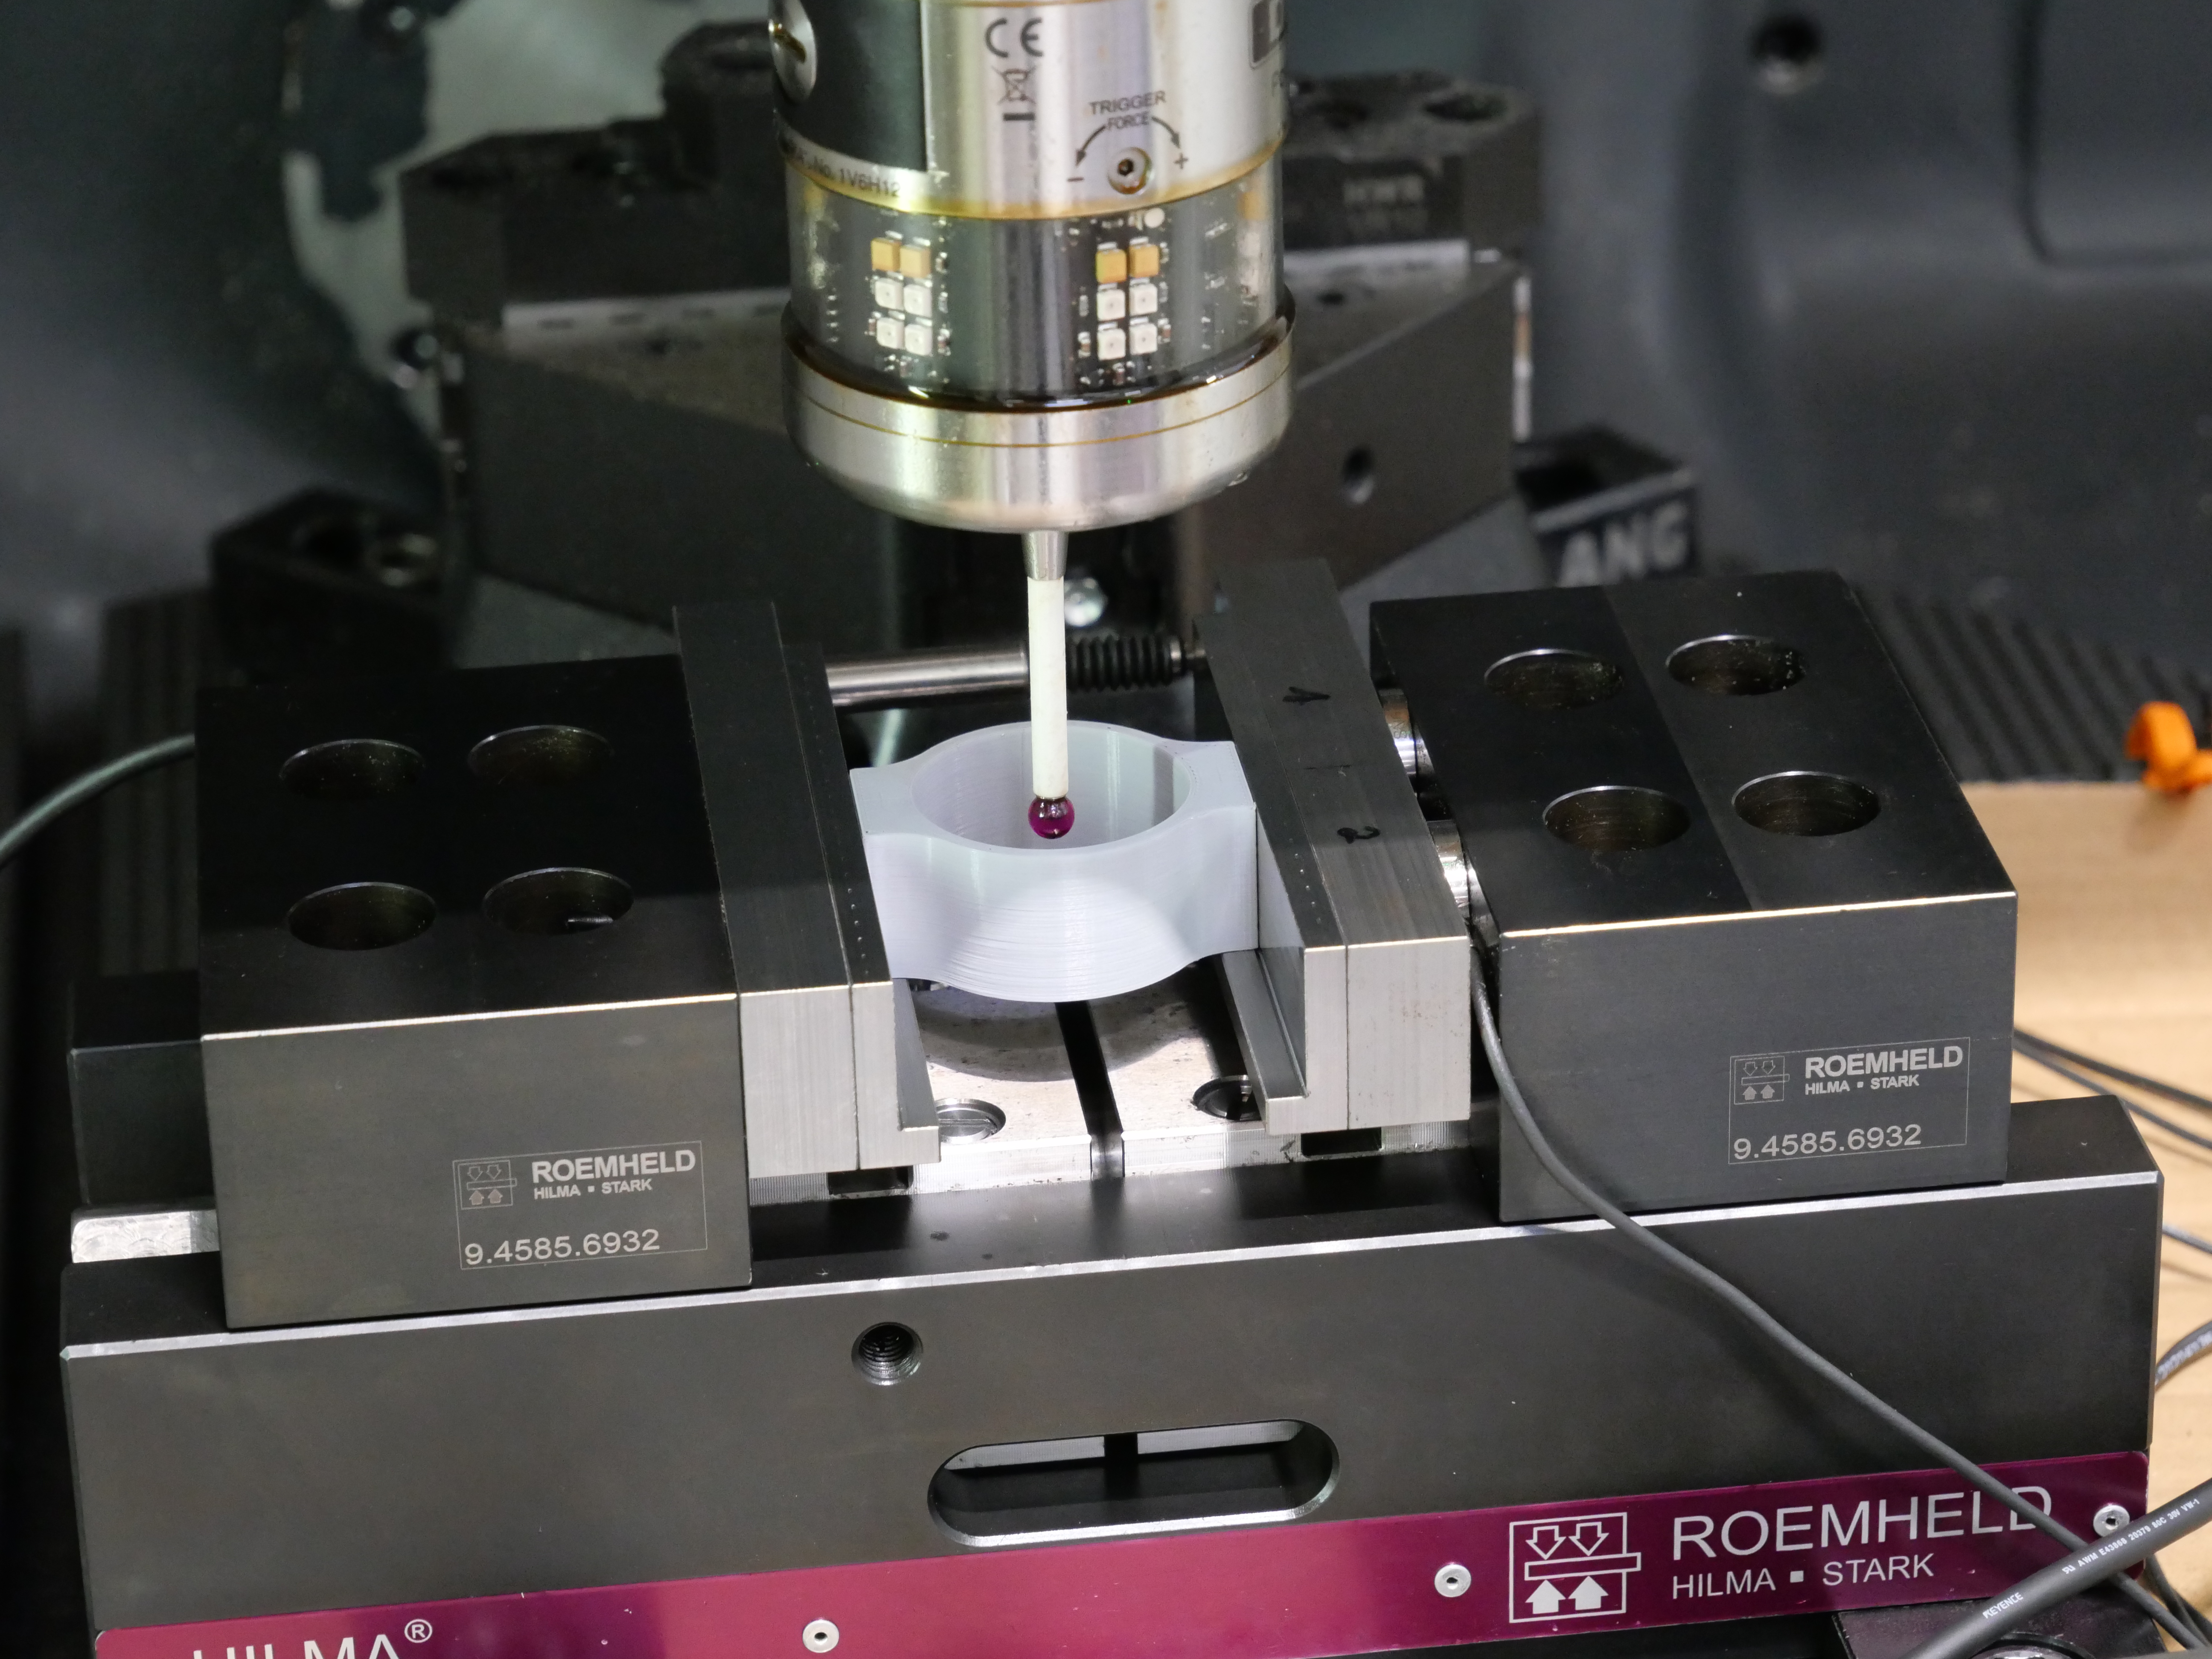
\includegraphics[width=0.4\textwidth]{images/taster.JPG}
    \caption{Taster}
    \label{fig:taster}
\end{figure}

\begin{figure}[b]
    \includegraphics[width=0.4\textwidth]{images/piezoelektrische.JPG}
    \caption{Spannungswandler}
    \label{fig:piez}
\end{figure}

Damit die Scanner Ergebnisse überprüft werden können,
wird die Bauteilgeometrie zusätzlich nach dem Scanvorgang noch mit einem Taster
abgetastet. Hierfür wird der Werkzeugkopf gewechselt und der Scanner entfernt.
Dann wird der Taster in die CNC-Maschine eingesetzt und das Bauteil abgetastet.
In Abbildung \ref{fig:taster} ist das Tasterwerkzeug zu sehen. Die rote Kugel 
am Ende des Tasters erkennt, sobald eine Berührung zu dem Bauteil erfolgt ist 
und benachrichtigt den Steuerungsrechner. Dieser speichert die aktuelle Position 
dann in einer Protokolldatei.

\end{document}